\documentclass[margin=0.1cm]{standalone}

%\usepackage{stix2}
\usepackage[]{tgheros}
\renewcommand{\familydefault}{\sfdefault}
\usepackage{arevmath}
\usepackage[italic]{mathastext}
\usepackage[T1]{fontenc}

\usepackage{pgfplots}
\pgfplotsset{compat=1.17}
\usepackage{siunitx}

\usepackage{booktabs}

\begin{document}
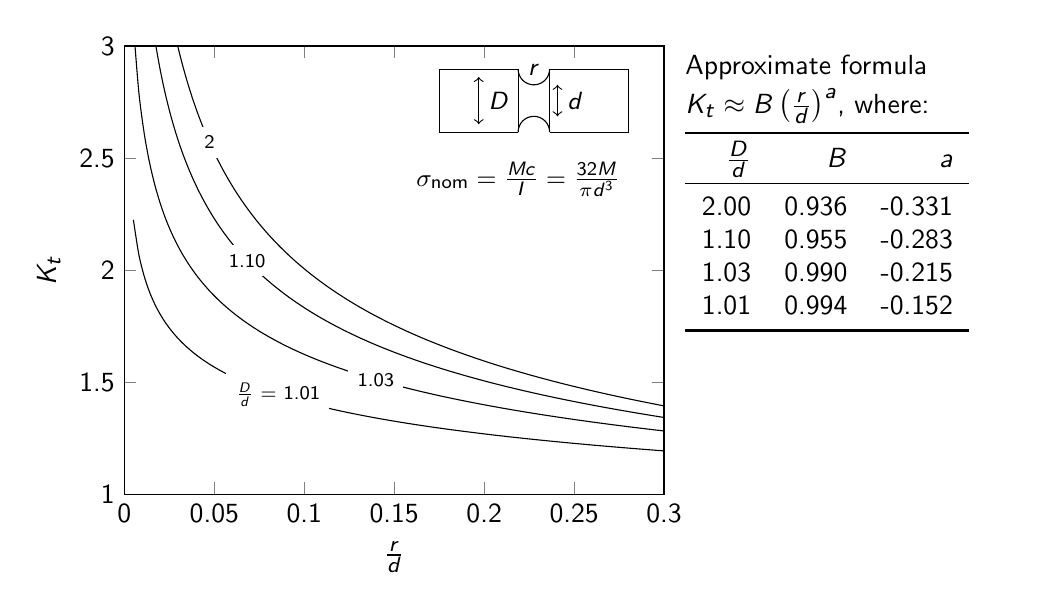
\begin{tikzpicture}
    \begin{axis}[
        xlabel = $\frac{r}{d}$,
        ylabel = $K_t$,
        ymin={1},
        ymax={3},
        xmin={0},
        xmax={0.3},
        x tick label style={
            /pgf/number format/.cd,
                fixed,
                %fixed zerofill,
                precision=2,
            /tikz/.cd
        },
        domain={0.005:0.3},
        samples={100}
    ]
    
    \addplot[smooth] {0.994*x^-0.152} node[pos=0.7, fill=white] {\scriptsize $\frac{D}{d}$ = 1.01};
    \addplot[smooth] {0.990*x^-0.215} node[pos=0.85, fill=white] {\scriptsize 1.03};
    \addplot[smooth] {0.955*x^-0.283} node[pos=0.75, fill=white] {\scriptsize 1.10};
    \addplot[smooth] {0.936*x^-0.331} node[pos=0.7, fill=white] {\scriptsize 2};

    
    \end{axis}
    
    %% Drawing (going clockwise from top left)
    
    \draw[] (4,5.4) -- (5,5.4);
    \draw (5,5.4) arc [start angle=180, end angle=360, x radius=0.2cm, y radius=0.2cm] node[pos=0.5, anchor=south] {\small $r$};
    \draw[] (5.4,5.4) -- ++(1, 0) -- ++ (0,-0.8) -- ++(-1, 0);
    \draw (5,4.6) arc [start angle=180, end angle=0, x radius=0.2cm, y radius=0.2cm];
    \draw[] (5.0,4.6) -- (4.0, 4.6);
    \draw[] (4.0, 4.6) -- (4, 5.4);
    
    \draw[] (5.0, 4.6) -- (5.0, 5.4);
    \draw[] (5.4, 4.6) -- (5.4, 5.4);
    
    \draw[<->] (4.5, 4.7) -- (4.5, 5.3) node[pos=0.5, anchor=west] {\small $D$};
    
    \draw[<->] (5.5, 4.8) -- (5.5, 5.2) node[pos=0.5, anchor=west] {\small $d$};

    \node[] at (5, 4) (maths) {\small$\sigma_\text{nom}=\frac{Mc}{I}=\frac{32M}{\pi{}d^3}$};
    
    %% Table %%
    
    \node[anchor=north west, text width=4cm] at (7, 5.7) (table) {
        Approximate formula \\[0.2em]
        $K_t\approx B\left(\frac{r}{d}\right)^a$, where:\\[0.2em]
        \begin{tabular}{rrr}
            \toprule
            $\frac{D}{d}$ & $B$ & $a$ \\
            \midrule
            2.00 & 0.936 & -0.331 \\
            1.10 & 0.955 & -0.283 \\
            1.03 & 0.990 & -0.215 \\
            1.01 & 0.994 & -0.152 \\
            \bottomrule
        \end{tabular}
    };
\end{tikzpicture}
\end{document}